\documentclass{article}
\usepackage{graphicx}
\usepackage{multirow}
\usepackage[utf8]{inputenc}
\usepackage{listings}
\usepackage{xcolor}
\usepackage{rotating}

\definecolor{codegreen}{rgb}{0,0.6,0}
\definecolor{codegray}{rgb}{0.5,0.5,0.5}
\definecolor{codepurple}{rgb}{0.58,0,0.82}
\definecolor{backcolour}{rgb}{0.95,0.95,0.92}

\lstdefinestyle{mystyle}{
	backgroundcolor=\color{backcolour},   
	commentstyle=\color{codegreen},
	keywordstyle=\color{magenta},
	numberstyle=\tiny\color{codegray},
	stringstyle=\color{codepurple},
	basicstyle=\ttfamily\footnotesize,
	breakatwhitespace=false,         
	breaklines=true,                 
	captionpos=b,                    
	keepspaces=true,                 
	numbers=left,                    
	numbersep=5pt,                  
	showspaces=false,                
	showstringspaces=false,
	showtabs=false,                  
	tabsize=2
}

\lstset{style=mystyle}

\usepackage[a4paper, total={6in, 8in}]{geometry}
\title{Assignment 1 Part 1 \\
		Analysis and Report}
\author{Student ID : 28993373\\
	Bhanuka Manesha Samarasekara Vitharana Gamage\\
	bsam0002@student.monash.edu\\
	School of Information Technology}

\begin{document}
	\lstset{language=Python}   
	\maketitle
	
	\section{Proof of the Heuristic Function}
	
	The \emph{input1.txt} example is shown below :
	
	\begin{figure}[!h]
		\centering
		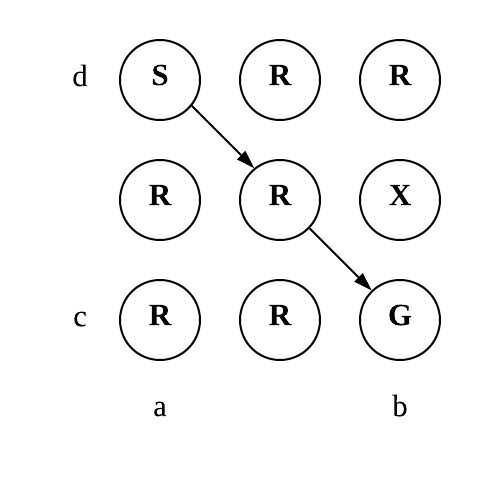
\includegraphics[width=50mm]{img1.png}
		\caption{Minimum Heuristic from Start to Goal for \emph{input1.txt}}
		\label{fig:img1}
	\end{figure}
	
	Using the above example, we will prove that the heuristic is valid. The heuristic used in this case is the maximum between the difference from the current state to the goal state. The derivation of $h(n)$ is stated below:
	
	\begin{equation} 
		dx = | b - a | \label{equation:2}
	\end{equation}
	\begin{equation} 
		dy = | d - c | \label{equation:3}
	\end{equation}
	
	\begin{equation}
		h(n) = max(dx,dy) \label{equation:4}
	\end{equation}
	
			\newpage
	Below is the python implementation for the heuristic:


		\begin{lstlisting}[language=Python]
		def heuristic(self,x,y):
			'''
			method used to calculate the heuristic value given the 
			current x and y coordinates
			@param x: current x coordinate
			@param y: current y coordinate
			@return: returns the heuristic value
			'''
			# Calculate the difference in both x and y directions
			dx = abs(x - self.GOAL_COORD[0])
			dy = abs(y - self.GOAL_COORD[1])
			
			# Returns the max of either the x or y direction
			return max(dx,dy)
		\end{lstlisting}

	 When determining the heuristic we assume that there are no ridges in the map. Therefore the rules are relaxed compared to the actual rules of the environment. 
	In order for the heuristic to be valid, it needs to be admissible and monotonic. Now let us prove that the above heuristic is Admissible and Monotonic.
	
	\subsection{Admissibility}
	
		In order for a heuristic to be admissible it needs to satisfy :
		\begin{equation}
			\forall n \quad h(n) \le h*(n) \label{equation:1}
		\end{equation}
				
		Since we get the maximum value between dx and dy as the heuristic, it will always be the minimum amount of diagonal moves between the start and goal state. Therefore we can deduce that all cost will be greater than the heuristic and will never be less than it. So for the best case the heuristic will be equal to the actual cost, but for the worst case the heuristic will be underestimating since the cost of non-diagonal moves are greater than one.
		
		Therefore the above heuristic is admissible as it satisfy Equation \ref{equation:1} and it does not overestimate the actual cost.
		
	\subsection{Monotonicity}
		In order for a heuristic to be monotonic, it should satisfy the following condition:
		\begin{equation}
			\forall n \quad h(n) \le c(m,n) + h(m) \label{equation:5}
		\end{equation}
		\begin{center}
			where m is a child of n
		\end{center}
	
	So rearranging the terms we can derive:
	\begin{equation}
		\forall n \quad h(n) - h(m)\le c(m,n)  \label{equation:6}
	\end{equation}

	Since the rules of the environment states that:
	\begin{equation}
		c(m,n) \ge 1
	\end{equation}
	
	and our heuristic will resolve:
	\begin{equation}
		h(n) - h(m) == 1
	\end{equation}
	
	thus satisfying equation \ref{equation:5}.
	
		\subsection{Is the resulting algorithm A or A*?}
		Since the actual cost is always used for the $g(n)$ value and not an estimate/ heuristic, we can state that the resulting algorithm is A*. 
		
	\section{Tie Breaker Implementation}
	
	As show below, to implement the tie breaker, we override the Node instance's less than operator:
			\begin{lstlisting}[language=Python]
    def __lt__(self, other):
			'''
			This method is used to override the less than operator in
			python to use the f cost for comparison
			@param other: the other node to be compared
			@return: boolean value stating whether its less than or not
			'''
			if (self.f < other.f):
				return True
			elif(self.f == other.f ):
				if self.operator in self.best_operators:
					return True
				elif other.operator in other.best_operators:
					return False
				else:
					return True
			else:
				return False
	\end{lstlisting}
	
	As per line 10, if the cost of the nodes are equal, we prioritize the node which was generated using a diagonal operator such as ``LU, LD, RU, RD''. So the tie breaker implementation will always prioritize paths with diagonals.
	
	\section{Test Cases}
	\subsection{Output for all the test cases}
		Below are the test cases and the resulting path from each algorithm:
		
		\subsubsection{input1.txt}
			\begin{lstlisting}
				3
				SRR
				RRX
				RRG
					
				DLS : S-RD-D-R-G 5
				A* : S-RD-D-R-G 5
		\end{lstlisting}
	\newpage
	\subsubsection{input2.txt}
		\begin{lstlisting}
				5
				SRRXG
				RXRXR
				RRRXR
				XRXRR
				RRRRX
				
				DLS : NO-PATH
				A* : S-D-D-R-D-D-R-R-U-R-U-U-U-G 24
		\end{lstlisting}
	
	\subsubsection{input3.txt}
		\begin{lstlisting}
				5
				SRXXX
				RRRXG
				XRRRR
				XRRRR
				RXXRX
		
				DLS : S-RD-RD-RD-RU-U-G 6
				A* :  S-RD-RD-RD-RU-U-G 6
		\end{lstlisting}
	
	\subsubsection{input4.txt}
		\begin{lstlisting}
				7
				RRRXRRR
				RXRRRXR
				RXXXXXR
				RRXSXXR
				XRXRXXR
				XRXRXXR
				XRRRXGR
				
				DLS : NO-PATH
				A* : S-D-D-D-L-L-U-U-U-L-U-U-U-R-R-D-R-R-U-R-R-D-D-D-D-D-D-L-G 54
		\end{lstlisting}
	
	\subsubsection{input5.txt}
		\begin{lstlisting}
				5
				SRRRG
				RRRRR
				XXXXX
				RRRRR
				RRRRR
				
				DLS : S-RD-R-R-RU-G 6
				A* : S-RD-RU-RD-RU-G 4
		\end{lstlisting}
		\newpage
	\subsubsection{input6.txt}
		\begin{lstlisting}
				10
				SRRRRRRRRR
				RRRRRRRRRR
				RRRRRRRRRR
				RRRRRRRRRR
				RRRRRRRRRR
				RRRRRRRRRR
				RRRRRRRRRR
				RRRRRRRRRR
				RRRRRRRRRR
				GRRRRRRRRR
				
				DLS : NO-PATH
				A* : S-RD-LD-RD-RD-LD-LD-RD-LD-D-G 10
		\end{lstlisting}

		\subsubsection{input7.txt}
	\begin{lstlisting}
				4
				XRGR
				SXRR
				RRXR
				RRRX
				
				
				DLS : NO-PATH
				A* : NO-PATH
	\end{lstlisting}
	
		\subsubsection{input8.txt}
	\begin{lstlisting}
				6
				SRRRRR
				RRRXXR
				RXRRRR
				RRXRXR
				XRRRRR
				GRRRXR
				
				DLS : NO-PATH
				A* : S-D-D-D-R-D-D-L-G 14
	\end{lstlisting}
	
	\subsubsection{input9.txt}
	\begin{lstlisting}
				6
				GRRRRR
				RRRRRR
				RRRRRR
				RRRRRR
				RRRRRR
				RRRRRS
				
				DLS : S-LU-LU-LU-LU-LU-G 5
				A* : S-LU-LU-LU-LU-LU-G 5
	\end{lstlisting}
	\newpage
	\subsection{Node expansion outputs}
	Below are the five node expansions for \emph{input1.txt}, \emph{input2.txt} and \emph{input3.txt} when using \textbf{A* algorithm}:
	
	\subsubsection{input1.txt}
	\begin{lstlisting}
	3
	SRR
	RRX
	RRG
	
	A* : S-RD-D-R-G 5
	
	N0:S    1 0 0 0
	Children:       {N1:S-R,N2:S-D,N3:S-RD}
	OPEN:   {(N3:S-RD 1 2 3)(N2:S-D 2 2 4)(N1:S-R 2 3 5)}
	CLOSED: {(N0:S 1 0 0 0)}
	
	N3:S-RD 2 1 2 3
	Children:       {N1:S-R,N2:S-D,N4:S-RD-LD,N5:S-RD-D}
	OPEN:   {(N4:S-RD-LD 2 2 4)(N2:S-D 2 2 4)(N5:S-RD-D 3 1 4)(N1:S-R 2 3 5)}
	CLOSED: {(N0:S 1 0 0 0)(N3:S-RD 2 1 2 3)}
	
	N4:S-RD-LD      3 2 2 4
	Children:       {N2:S-D,N5:S-RD-D}
	OPEN:   {(N5:S-RD-D 3 1 4)(N2:S-D 2 2 4)(N1:S-R 2 3 5)}
	CLOSED: {(N0:S 1 0 0 0)(N3:S-RD 2 1 2 3)(N4:S-RD-LD 3 2 2 4)}
	
	N5:S-RD-D       4 3 1 4
	Children:       {N2:S-D,N4:S-RD-LD,N6:S-RD-D-R-G}
	OPEN:   {(N2:S-D 2 2 4)(N1:S-R 2 3 5)(N6:S-RD-D-R-G 5 1 6)}
	CLOSED: {(N0:S 1 0 0 0)(N3:S-RD 2 1 2 3)(N4:S-RD-LD 3 2 2 4)(N5:S-RD-D 4 3 1 4)}
	
	N2:S-D  5 2 2 4
	Children:       {N1:S-R,N3:S-RD,N4:S-RD-LD,N5:S-RD-D}
	OPEN:   {(N1:S-R 2 3 5)(N6:S-RD-D-R-G 5 1 6)}
	CLOSED: {(N0:S 1 0 0 0)(N3:S-RD 2 1 2 3)(N4:S-RD-LD 3 2 2 4)(N5:S-RD-D 4 3 1 4)(N2:S-D 5 2 2 4)}

	\end{lstlisting}
	\newpage
	\subsubsection{input2.txt}
	\begin{lstlisting}
	5
	SRRXG
	RXRXR
	RRRXR
	XRXRR
	RRRRX
	
	A* : S-D-D-R-D-D-R-R-U-R-U-U-U-G 24
	
	N0:S    1 0 0 0
	Children:       {N1:S-R,N2:S-D}
	OPEN:   {(N1:S-R 2 3 5)(N2:S-D 2 4 6)}
	CLOSED: {(N0:S 1 0 0 0)}
	
	N1:S-R  2 2 3 5
	Children:       {N3:S-R-R}
	OPEN:   {(N2:S-D 2 4 6)(N3:S-R-R 4 2 6)}
	CLOSED: {(N0:S 1 0 0 0)(N1:S-R 2 2 3 5)}
	
	N2:S-D  3 2 4 6
	Children:       {N4:S-D-D}
	OPEN:   {(N3:S-R-R 4 2 6)(N4:S-D-D 4 4 8)}
	CLOSED: {(N0:S 1 0 0 0)(N1:S-R 2 2 3 5)(N2:S-D 3 2 4 6)}
	
	N3:S-R-R        4 4 2 6
	Children:       {N5:S-R-R-D}
	OPEN:   {(N4:S-D-D 4 4 8)(N5:S-R-R-D 6 2 8)}
	CLOSED: {(N0:S 1 0 0 0)(N1:S-R 2 2 3 5)(N2:S-D 3 2 4 6)(N3:S-R-R 4 4 2 6)}
	
	N4:S-D-D        5 4 4 8
	Children:       {N6:S-D-D-R}
	OPEN:   {(N5:S-R-R-D 6 2 8)(N6:S-D-D-R 6 3 9)}
	CLOSED: {(N0:S 1 0 0 0)(N1:S-R 2 2 3 5)(N2:S-D 3 2 4 6)(N3:S-R-R 4 4 2 6)(N4:S-D-D 5 4 4 8)}
	
	
	\end{lstlisting}
	\newpage
	\subsubsection{input3.txt}
	\begin{lstlisting}
	5
	SRXXX
	RRRXG
	XRRRR
	XRRRR
	RXXRX
	
	A* : S-RD-RD-RD-RU-U-G 6
	
	N0:S    1 0 0 0
	Children:       {N1:S-R,N2:S-D,N3:S-RD}
	OPEN:   {(N3:S-RD 1 3 4)(N1:S-R 2 3 5)(N2:S-D 2 4 6)}
	CLOSED: {(N0:S 1 0 0 0)}
	
	N3:S-RD 2 1 3 4
	Children:       {N1:S-R,N2:S-D,N4:S-RD-R,N5:S-RD-D,N6:S-RD-RD}
	OPEN:   {(N6:S-RD-RD 2 2 4)(N1:S-R 2 3 5)(N4:S-RD-R 3 2 5)(N2:S-D 2 4 6)(N5:S-RD-D 3 3 6)}
	CLOSED: {(N0:S 1 0 0 0)(N3:S-RD 2 1 3 4)}
	
	N6:S-RD-RD      3 2 2 4
	Children:       {N4:S-RD-R,N5:S-RD-D,N7:S-RD-RD-R,N8:S-RD-RD-LD,N9:S-RD-RD-D,N10:S-RD-RD-RD}
	OPEN:   {(N10:S-RD-RD-RD 3 1 4)(N4:S-RD-R 3 2 5)(N1:S-R 2 3 5)(N7:S-RD-RD-R 4 1 5)(N8:S-RD-RD-LD 3 3 6)(N5:S-RD-D 3 3 6)(N2:S-D 2 4 6)(N9:S-RD-RD-D 4 2 6)}
	CLOSED: {(N0:S 1 0 0 0)(N3:S-RD 2 1 3 4)(N6:S-RD-RD 3 2 2 4)}
	
	N10:S-RD-RD-RD  4 3 1 4
	Children:       {N7:S-RD-RD-R,N11:S-RD-RD-RD-RU,N9:S-RD-RD-D,N12:S-RD-RD-RD-R,N13:S-RD-RD-RD-D}
	OPEN:   {(N11:S-RD-RD-RD-RU 4 0 4)(N7:S-RD-RD-R 4 1 5)(N1:S-R 2 3 5)(N4:S-RD-R 3 2 5)(N8:S-RD-RD-LD 3 3 6)(N9:S-RD-RD-D 4 2 6)(N2:S-D 2 4 6)(N5:S-RD-D 3 3 6)(N12:S-RD-RD-RD-R 5 1 6)(N13:S-RD-RD-RD-D 5 2 7)}
	CLOSED: {(N0:S 1 0 0 0)(N3:S-RD 2 1 3 4)(N6:S-RD-RD 3 2 2 4)(N10:S-RD-RD-RD 4 3 1 4)}
	
	N11:S-RD-RD-RD-RU       5 4 0 4
	Children:       {N14:S-RD-RD-RD-RU-U-G,N7:S-RD-RD-R,N12:S-RD-RD-RD-R}
	OPEN:   {(N4:S-RD-R 3 2 5)(N1:S-R 2 3 5)(N7:S-RD-RD-R 4 1 5)(N8:S-RD-RD-LD 3 3 6)(N12:S-RD-RD-RD-R 5 1 6)(N5:S-RD-D 3 3 6)(N2:S-D 2 4 6)(N9:S-RD-RD-D 4 2 6)(N13:S-RD-RD-RD-D 5 2 7)(N14:S-RD-RD-RD-RU-U-G 6 1 7)}
	CLOSED: {(N0:S 1 0 0 0)(N3:S-RD 2 1 3 4)(N6:S-RD-RD 3 2 2 4)(N10:S-RD-RD-RD 4 3 1 4)(N11:S-RD-RD-RD-RU 5 4 0 4)}

	\end{lstlisting}
	\newpage
	\section{Analysis for test maps}
	In order to perform an analysis, multiple test cases were generated and tested on the two algorithms. Below is a table with the time taken for each input by the two algorithms. Please do note that each time is an \textbf{average of five runs} and the \textbf{bound of the DLS is set to 5}.
	
	\begin{table}[!h] 
		\scalebox{0.7}{
		\begin{tabular}{|c|c|l|l|l|l|l|l|l|l|l|l|l|}
			\hline
			\multirow{3}{*}{\textbf{Input File}} & \multicolumn{12}{c|}{\textbf{Time Taken}}                                                                   \\ \cline{2-13} 
			& \multicolumn{6}{c|}{\textbf{DLS}}                                        & \multicolumn{6}{c|}{\textbf{A*}} \\ \cline{2-13} 
			& \multicolumn{1}{l|}{1} & 2                         & 3 & 4 & 5 & \textbf{Average} & 1  & 2  & 3  & 4  & 5  & \textbf{Average}  \\ \hline
			input1.txt                           &0.00024 &	0.00017&	0.00023&	0.00017&	0.00017&	\textbf{0.00020}	&0.00028&	0.00028&	0.00028	&0.00033&	0.00028&	\textbf{0.00029 }   \\ \hline
			
			input2.txt                           & 0.00037	& 0.00036	&0.00037&	0.00038&	0.00037	&\textbf{0.00037}&	0.00132&	0.00090&	0.00092	&0.00083&	0.00083&\textbf{	0.00096  }   \\ \hline
			
			input3.txt                           & 0.00035&	0.00034&	0.00035	&0.00035&	0.00035	&\textbf{0.00035}	&0.00081&	0.00068	&0.00058&	0.00057	&0.00057&	\textbf{0.00064     }\\ \hline
			
			input4.txt                           & 0.00023 &	0.00022&	0.00023	&0.00023&	0.00024&	\textbf{0.00023}	&0.00152&	0.00152&	0.00150&	0.00152&	0.00150&\textbf{	0.00151 }   \\ \hline
			
			input5.txt                           & 0.00035 &	0.00027	& 0.00027	&0.00027	& 0.00027	&\textbf{0.00029}	&0.00029	&0.00029	&0.00028	&0.00027& 	0.00029	&\textbf{0.00028 }   \\ \hline
			
			input6.txt                           & 0.00201	&0.00197&	0.00202&	0.00198	&0.00197&	\textbf{0.00199}&	0.00336&	0.00373&	0.00369 &	0.00446 &	0.00431& 	\textbf{0.00385   }\\ \hline
			
			input7.txt                           & 0.00026	& 0.00021& 	0.00023& 	0.00022	& 0.00022& 	\textbf{0.00023}& 	0.00022& 	0.00026& 	0.00023	& 0.00023	& 0.00023	& \textbf{0.00023   } \\ \hline
			
			input8.txt                           & 0.00061	&0.00059&	0.00049&	0.00049	&0.00050&\textbf{0.00054}	&0.00081&	0.00082	&0.00087&	0.00083	&0.00083&	\textbf{0.00083 }   \\ \hline
			
			input9.txt                           & 0.00349	&0.00347&	0.00349&	0.00349&	0.00347&	\textbf{0.00348}&	0.00077	&0.00078&	0.00094	&0.00078&	0.00077&	\textbf{0.00080}   \\ \hline
		\end{tabular}
	}
	 \caption{Time Taken for each Algorithm on each input file}
	 \label{T1}
	\end{table}

	Now let us analyze the results for each test map. For all the analysis, we considered a bound of 5 for DLS. The reason for this is to test the boundary cases where the only path for DLS is the optimal path. So for some of the cases, the there will be no solution as DLS is not complete.
	
	\subsection{input1.txt}
		\begin{lstlisting}
		3
		SRR
		RRX
		RRG
		
		DLS : S-RD-D-R-G 5
		A* : S-RD-D-R-G 5
		\end{lstlisting}
		
		In this test case, both the DLS and A* perform equally. The reason for this is the graph search updates the cost of the nodes in the open list to the nodes with the minimum cost to a certain location. So if the DLS get an expensive path to a node, it is not updated. Therefore, in DLS, if the correct actions are picked first, both of them can perform equally and can lead to an optimal path. But A* will guarantee an optimal path but will take more time. So from Table \ref{T1} we can see that for \emph{input1.txt} on average A* was slower.\newline
		
	\newpage
	\subsection{input2.txt}
		\begin{lstlisting}
		5
		SRRXG
		RXRXR
		RRRXR
		XRXRR
		RRRRX
		
		DLS : NO-PATH
		A* : S-D-D-R-D-D-R-R-U-R-U-U-U-G 24
		\end{lstlisting}
		
		In this test case, DLS returns NO-PATH since the depth of the optimal solution is more than 6. So there is no path for DLS to reach the goal in less than 5 steps. This shows that DLS is not complete. \newline
	
	\subsection{input3.txt}	
		\begin{lstlisting}
		5
		SRXXX
		RRRXG
		XRRRR
		XRRRR
		RXXRX
		
		DLS : S-RD-RD-RD-RU-U-G 6
		A* :  S-RD-RD-RD-RU-U-G 6
		\end{lstlisting}
		
		Similar to \emph{input1.txt}, DLS also returns the optimal path and A* takes more time to run. This map was used to test how the agent react to when it finds a shorter path at the last step. So if the agent stopped when the goal node was generated, we would get an error as there is a better path than the initial path.\newline
		
	\subsection{input4.txt}	
		\begin{lstlisting}
		7
		RRRXRRR
		RXRRRXR
		RXXXXXR
		RRXSXXR
		XRXRXXR
		XRXRXXR
		XRRRXGR
		
		DLS : NO-PATH
		A* : S-D-D-D-L-L-U-U-U-L-U-U-U-R-R-D-R-R-U-R-R-D-D-D-D-D-D-L-G 54
		\end{lstlisting}
	Similar to \emph{input2.txt}, DLS returns NO-PATH and A* takes more time to run. This map is used to test whether the agent follows the rules of the environment and not choose paths out of bounds. \newline

	\newpage
	\subsection{input5.txt}	
		\begin{lstlisting}
		5
		SRRRG
		RRRRR
		XXXXX
		RRRRR
		RRRRR
		
		DLS : S-RD-R-R-RU-G 6
		A* : S-RD-RU-RD-RU-G 4
		\end{lstlisting}
		The ridges blocks the bottom half of the map. So this map is useful in testing whether the agent takes the shorter path or the longer path to get to the goal. This also test whether the rules of the environment are stable. The run time of both algorithms are similar since the optimal path is similar to a DLS, where picking the diagonals is the best option.But as the results indicate, DLS takes a longer, non optimal path compared to A*.This is due to the order of actions taken by the agent. \newline
	
	\subsection{input6.txt}	
		\begin{lstlisting}
		10
		SRRRRRRRRR
		RRRRRRRRRR
		RRRRRRRRRR
		RRRRRRRRRR
		RRRRRRRRRR
		RRRRRRRRRR
		RRRRRRRRRR
		RRRRRRRRRR
		RRRRRRRRRR
		GRRRRRRRRR
		
		DLS : NO-PATH
		A* : S-RD-LD-RD-RD-LD-LD-RD-LD-D-G 10
		\end{lstlisting}
		This test can be used to see if the agent chooses the most optimal path, as taking diagonal actions only doesn't lead to the goal node. The run time of A* is more because DLS is bounded to 5.  \newline
	
	\subsection{input7.txt}	
		\begin{lstlisting}
		4
		XRGR
		SXRR
		RRXR
		RRRX
		
		
		DLS : NO-PATH
		A* : NO-PATH
		\end{lstlisting}
		This test map was used to test how the agent handles, when there is no path to the goal. So both agents returned NO-PATH, with equal run time as they had to exhaust all the paths. \newline
	
	\subsection{input8.txt}	
		\begin{lstlisting}
		6
		SRRRRR
		RRRXXR
		RXRRRR
		RRXRXR
		XRRRRR
		GRRRXR
		
		DLS : NO-PATH
		A* : S-D-D-D-R-D-D-L-G 14
		\end{lstlisting}
		This test map was used to test how the agent handles, when there is a shorter path with more horizontal moves than diagonal moves. So the DLS did not find a path while A* found the path while taking more run time. \newline
		
	\subsection{input9.txt}	
		\begin{lstlisting}
		6
		GRRRRR
		RRRRRR
		RRRRRR
		RRRRRR
		RRRRRR
		RRRRRS
		
		DLS : S-LU-LU-LU-LU-LU-G 5
		A* : S-LU-LU-LU-LU-LU-G 5
		\end{lstlisting}
		This test map was used to test how the agent handles, when the Start and Goal nodes are swapped with no obstacles. Another constraint is the path for DLS is the same length as the bound. So the DLS should return the most optimal path. So looking at the results, we see that the DLS takes more time compared to A*. This is because the A* algoritm only used 5 moves and gets to the goal node, where as DLS has to go through all the possible paths upto the bound until it finds the single optimal path.\newline
	\section{Conclusion}
	Therefore in conclusion we can see that the A* algorithm finds the optimal path compared to DLS, while DLS is faster at finding paths. But if the path is outside the bound value, DLS doesn't find the path. Therefore DLS is not complete while on the other hand, A*, given that there exist a path will always find it.
	
\end{document}